% Created 2019-12-08 Sun 22:26
% Intended LaTeX compiler: pdflatex
\documentclass[11pt,titlepage]{article}
\usepackage[utf8x]{inputenc}
\usepackage[T1]{fontenc}
\usepackage{graphicx}
\usepackage{grffile}
\usepackage{longtable}
\usepackage{wrapfig}
\usepackage{rotating}
\usepackage[normalem]{ulem}
\usepackage{amsmath}
\usepackage{textcomp}
\usepackage{amssymb}
\usepackage{capt-of}
\usepackage{hyperref}
\usepackage[a4paper,total={6.5in, 9.5in}]{geometry}
\usepackage{libertine}
\usepackage{pdfpages}
\usepackage{minted}
\setminted{fontsize=\footnotesize}
\usepackage[font={small,sf},labelfont=bf,format=hang,format=plain,margin=0pt,width=0.8\textwidth,]{caption}
\usepackage[list=true]{subcaption}
\author{Jakub Zárybnický, xzaryb00}
\date{6. 12. 2019}
\title{Projekt z MSP\\\medskip
\large Logo VUT! VYSOKÉ UČENÍ TECHNICKÉ V BRNĚ Fakulta informačních technologií Čísla zadání: 21, 6 Cvičení - skupina: pátek, 9.00}
\hypersetup{
 pdfauthor={Jakub Zárybnický, xzaryb00},
 pdftitle={Projekt z MSP},
 pdfkeywords={},
 pdfsubject={},
 pdfcreator={Emacs 26.1 (Org mode 9.1.9)}, 
 pdflang={Czech}}
\begin{document}


\includepdf{title-page.pdf}

\section{Zadání projektu z předmětu MSP}
\label{sec:orgd7a26e9}
\textbf{Každý student obdrží na cvičení konkrétní data (čísla ze seznamu), pro které vypracuje projekt.}
K vypracování můžete použít libovolné statistické programy.

\begin{enumerate}
\item Při kontrole výrobků byla sledována odchylka X [mm] jejich rozměru od
požadované velikosti. Naměřené hodnoty tvoří statistický soubor v listu
Data př. 1.

\begin{enumerate}
\item Proveďte roztřídění statistického souboru, vytvořte tabulku četností a
nakreslete histogramy pro relativní četnosti a relativní kumulativní
četnosti.
\item Vypočtěte aritmetický průměr, medián, modus, rozptyl a směrodatnou
odchylku.
\item Vypočtěte bodové odhady střední hodnoty, rozptylu a směrodatné odchylky.
\item Testujte předpoklad o výběru z normálního rozdělení Pearsonovým
(chí-kvadrát) testem na hladině významnosti 0,05.
\item Za předpokladu (bez ohledu na výsledek části d)), že statistický soubor
byl získán náhodným výběrem z normálního rozdělení, určete intervalové
odhady střední hodnoty, rozptylu a směrodatné odchylky se spolehlivostí
0,95 a 0,99.
\item Testujte hypotézu optimálního seřízení stroje, tj. že střední hodnota
odchylky je nulová, proti dvoustranné alternativní hypotéze, že střední
hodnota odchylky je různá od nuly, a to na hladině významnosti 0,05.
\item Ověřte statistickým testem na hladině významnosti 0,05, zda seřízení
stroje ovlivnilo kvalitu výroby, víte-li, že výše uvedený statistický
soubor 50-ti hodnot vznikl spojením dvou dílčích statistických souborů
tak, že po naměření prvních 20-ti hodnot bylo provedeno nové seřízení
stroje a pak bylo naměřeno zbývajících 30 hodnot.
\end{enumerate}

Návod: Oba soubory zpracujte neroztříděné. Testujte nejprve rovnost rozptylů
odchylek před a po seřízení stroje. Podle výsledku pak zvolte vhodný postup
pro testování rovnosti středních hodnot odchylek před a po seřízení stroje.

\item Měřením dvojice (Výška[cm], Váha[kg]) u vybraných studentů z FIT byl získán
dvourozměrný statistický soubor zapsaný po dvojicích v řádcích v listu
Data př. 2.

\begin{enumerate}
\item Vypočtěte bodový odhad koeficientu korelace.
\item Na hladině významnosti 0,05 testujte hypotézu, že náhodné veličiny Výška a
Váha jsou lineárně nezávislé.
\item \textbf{Regresní analýza} - data proložte přímkou: \(Vaha = \beta_0 + \beta_1 \times Vyska\)
\begin{enumerate}
\item Bodově odhadněte \(\beta_0\), \(\beta_1\) a rozptyl \(s_2\).
\item Na hladině významnosti 0,05 otestujte hypotézy:
\[H : \beta_0 = -100, H_A : \beta_0 \neq -100,\]
\[H : \beta_1 = 1, H_A : \beta_1 \neq 1,\]
\item Vytvořte graf bodů spolu s regresní přímkou a pásem spolehlivosti pro
individuální hodnotu výšky.
\end{enumerate}
\end{enumerate}
\end{enumerate}

\textbf{Termín pro odevzdání práce je 11. týden výuky zimního semestru ve cvičení.}

\newpage

\begin{listing}[htbp]
\begin{minted}[]{python}
%matplotlib inline
import matplotlib.gridspec as gridspec
import matplotlib.pyplot as plt
import numpy as np
import pandas as pd
from scipy.stats import chi2, f, norm, t
from tabulate import tabulate

def show(*args, headers='keys', **kwargs):
    print(tabulate(*args, tablefmt='orgtbl', headers=headers, **kwargs))

ex1 = pd.DataFrame(ex1_raw, columns=['odchylka'])
ex2 = pd.DataFrame(ex2_raw, columns=['vyska', 'vaha'])
\end{minted}
\end{listing}

\section{Příklad 1}
\label{sec:org03d4000}
\textbf{Při kontrole výrobků byla sledována odchylka X [mm] jejich rozměru od požadované velikosti.
Naměřené hodnoty tvoří statistický soubor v listu Data př. 1.}

\begin{figure}[htbp]\centering\begin{subfigure}[t]{0.5\textwidth}\centering\begin{subfigure}[t]{0.5\textwidth}
\begin{center}
\begin{tabular}{rr}
 & Odchylka [mm]\\
\hline
1 & 1.83\\
2 & 0.98\\
3 & -0.09\\
4 & -0.23\\
5 & 2.56\\
6 & 0.31\\
7 & 1.06\\
8 & 0.01\\
9 & 0.75\\
10 & 2.26\\
11 & -0.59\\
12 & 0.9\\
13 & 1.66\\
14 & 0.36\\
15 & 2.19\\
16 & 1.24\\
17 & -0.58\\
18 & 0.79\\
19 & 0.02\\
20 & 0.31\\
21 & 1.61\\
22 & 0.75\\
23 & 2.46\\
24 & 0.86\\
25 & 0.63\\
\end{tabular}
\end{center}
\end{subfigure}~\begin{subfigure}[t]{0.5\textwidth}
\begin{center}
\begin{tabular}{rr}
 & Odchylka [mm]\\
\hline
26 & -0.98\\
27 & -0.75\\
28 & 2.67\\
29 & 1.79\\
30 & 1.84\\
31 & 0.49\\
32 & 1.68\\
33 & 0.39\\
34 & -0.84\\
35 & 1.49\\
36 & 1.5\\
37 & 1.7\\
38 & 3.4\\
39 & 1.4\\
40 & 0.27\\
41 & 0.48\\
42 & 0.27\\
43 & 1.41\\
44 & 0.55\\
45 & 1.2\\
46 & -0.68\\
47 & 1.59\\
48 & 0.8\\
49 & 1.21\\
50 & -1.31\\
\end{tabular}
\end{center}
\end{subfigure}\caption{Statistický soubor}\end{subfigure}~
\hfill\begin{subfigure}[t]{0.5\textwidth}\centering\begin{subfigure}[t]{0.5\textwidth}
\begin{center}
\begin{tabular}{lr}
 & Odchylka [mm]\\
\hline
(1) & -1.31\\
(2) & -0.98\\
(3) & -0.84\\
(4) & -0.75\\
(5) & -0.68\\
(6) & -0.59\\
(7) & -0.58\\
(8) & -0.23\\
(9) & -0.09\\
(10) & 0.01\\
(11) & 0.02\\
(12) & 0.27\\
(13) & 0.27\\
(14) & 0.31\\
(15) & 0.31\\
(16) & 0.36\\
(17) & 0.39\\
(18) & 0.48\\
(19) & 0.49\\
(20) & 0.55\\
(21) & 0.63\\
(22) & 0.75\\
(23) & 0.75\\
(24) & 0.79\\
(25) & 0.8\\
\end{tabular}
\end{center}
\end{subfigure}~\begin{subfigure}[t]{0.5\textwidth}
\begin{center}
\begin{tabular}{lr}
 & Odchylka [mm]\\
\hline
(26) & 0.86\\
(27) & 0.9\\
(28) & 0.98\\
(29) & 1.06\\
(30) & 1.2\\
(31) & 1.21\\
(32) & 1.24\\
(33) & 1.4\\
(34) & 1.41\\
(35) & 1.49\\
(36) & 1.5\\
(37) & 1.59\\
(38) & 1.61\\
(39) & 1.66\\
(40) & 1.68\\
(41) & 1.7\\
(42) & 1.79\\
(43) & 1.83\\
(44) & 1.84\\
(45) & 2.19\\
(46) & 2.26\\
(47) & 2.46\\
(48) & 2.56\\
(49) & 2.67\\
(50) & 3.4\\
\end{tabular}
\end{center}
\end{subfigure}\caption{Uspořádaný statistický soubor}\end{subfigure}\end{figure}

\subsection{Proveďte roztřídění statistického souboru, vytvořte tabulku četností a nakreslete histogramy pro relativní četnosti a relativní kumulativní četnosti.}
\label{sec:orga08d732}

\begin{listing}[htbp]
\begin{minted}[]{python}
categories, bins = pd.cut(ex1.odchylka, bins=11, retbins=True)
print('\nBin size:' , bins[1] - bins[0], end='\n\n')
tbl, cumsum = [], 0
for ix, (bin, cnt) in enumerate(categories.value_counts(sort=False).items()):
  cumsum += cnt
  tbl.append([ix + 1, bin,
              str((bin.right - bin.left) / 2 + bin.left),
              cnt, cumsum,
              cnt / len(categories), cumsum / len(categories)])
show(tbl, headers=["Třída", "Okraje", "Střed", "Četnost", "Kum. četnost",
                   "Rel. četnost", "Rel. kum. četnost"])
\end{minted}
\end{listing}



Bin size: 0.4328918181818182

\begin{center}
\begin{tabular}{rlrrrrr}
Třída & Okraje & Střed & Četnost & Kum. četnost & Rel. četnost & Rel. kum. četnost\\
\hline
1 & (-1.315, -0.882] & -1.0985 & 2 & 2 & 0.04 & 0.04\\
2 & (-0.882, -0.454] & -0.668 & 5 & 7 & 0.1 & 0.14\\
3 & (-0.454, -0.0255] & -0.23975 & 2 & 9 & 0.04 & 0.18\\
4 & (-0.0255, 0.403] & 0.18875 & 8 & 17 & 0.16 & 0.34\\
5 & (0.403, 0.831] & 0.617 & 8 & 25 & 0.16 & 0.5\\
6 & (0.831, 1.259] & 1.045 & 7 & 32 & 0.14 & 0.64\\
7 & (1.259, 1.687] & 1.473 & 8 & 40 & 0.16 & 0.8\\
8 & (1.687, 2.115] & 1.901 & 4 & 44 & 0.08 & 0.88\\
9 & (2.115, 2.544] & 2.3295 & 3 & 47 & 0.06 & 0.94\\
10 & (2.544, 2.972] & 2.758 & 2 & 49 & 0.04 & 0.98\\
11 & (2.972, 3.4] & 3.186 & 1 & 50 & 0.02 & 1\\
\end{tabular}
\end{center}

\newpage

\begin{listing}[htbp]
\begin{minted}[]{python}
freq = categories.value_counts(sort=False).reset_index().odchylka
plt.figure(figsize=(8, 4))
plt.subplot(1, 2, 1); _ = freq.plot.bar()
plt.subplot(1, 2, 2); _ = freq.cumsum().plot.bar()
plt.tight_layout(); plt.show()
\end{minted}
\end{listing}

\begin{center}
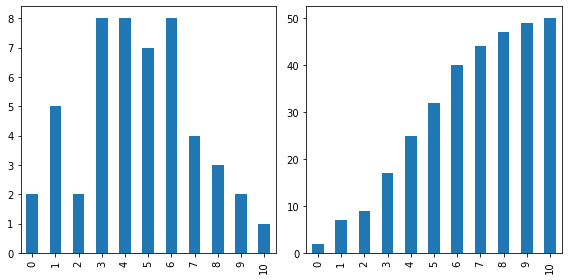
\includegraphics[width=.9\linewidth]{./obipy-resources/qPqHVY.png}
\end{center}

\subsection{Vypočtěte aritmetický průměr, medián, modus, rozptyl a směrodatnou odchylku.}
\label{sec:orgac4b344}
\begin{listing}[htbp]
\begin{minted}[]{python}
show({'mean':   [ex1.odchylka.mean()],
      'median': [ex1.median()],
      'mode':   [', '.join(map(str, ex1.odchylka.mode()))],
      'var':    [ex1.var()],
      'std':    [ex1.std()]})
\end{minted}
\end{listing}

\begin{center}
\begin{tabular}{rrlrr}
mean & median & mode & var & std\\
\hline
0.8724 & 0.83 & 0.27, 0.31, 0.75 & 1.07134 & 1.03506\\
\end{tabular}
\end{center}

\subsection{Vypočtěte bodové odhady střední hodnoty, rozptylu a směrodatné odchylky.}
\label{sec:org397e7d4}

\begin{listing}[htbp]
\begin{minted}[]{python}
show({'mean': [ex1.odchylka.mean()],
      'var':  [ex1.odchylka.var()],
      'std':  [ex1.odchylka.std()]})
\end{minted}
\end{listing}

\begin{center}
\begin{tabular}{rrr}
mean & var & std\\
\hline
0.8724 & 1.07134 & 1.03506\\
\end{tabular}
\end{center}
\newpage

\subsection{Testujte předpoklad o výběru z normálního rozdělení Pearsonovým (chí-kvadrát) testem na hladině významnosti 0,05}
\label{sec:org9a919a2}

\begin{listing}[htbp]
\begin{minted}[]{python}
bins = [-1000, -0.6, 0.1, 0.4, 0.8, 1.2, 1.49, 1.68, 2.2, 1000]
test_categories = pd.cut(ex1.odchylka, bins=bins)
tbl, cumsum = [], 0
diffs = []
p_exp = norm(loc=ex1.odchylka.mean(), scale=ex1.odchylka.std())
for ix, (bin, cnt) in enumerate(test_categories.value_counts(sort=False).items()):
  cumsum += cnt
  middle = (bin.right - bin.left) / 2 + bin.left
  expect = abs(p_exp.cdf(bin.right) - p_exp.cdf(bin.left)) * len(categories)
  diff = (cnt - expect) ** 2 / expect
  diffs.append(diff)
  tbl.append([ix + 1, bin, str(middle), cumsum, cnt, expect, diff])
show(tbl, headers=["Třída", "Okraje", "Střed", "Kum. četnost", "Četnost",
                   "Teor.čet", "Rozd^2/teor.čet"])
print("\nCriterium =", sum(diffs))
pval = chi2.ppf(0.95, df=len(diffs) - 2 - 1)
print("\nChi-squared(0.95) =", pval)
print("\nCritical region complement = [0, %s]" % pval)
print("\nThe test criterium falls within this region, "
      "therefore we don't reject the hypothesis.")
\end{minted}
\end{listing}

\begin{center}
\begin{tabular}{rlrrrrr}
Třída & Okraje & Střed & Kum. četnost & Četnost & Teor.čet & Rozd\(^{\text{2}}\)/teor.čet\\
\hline
1 & (-1000.0, -0.6] & -500.3 & 5 & 5 & 3.8718 & 0.328746\\
2 & (-0.6, 0.1] & -0.25 & 11 & 6 & 7.51627 & 0.305878\\
3 & (0.1, 0.4] & 0.25 & 17 & 6 & 4.81449 & 0.291919\\
4 & (0.4, 0.8] & 0.6 & 25 & 8 & 7.40333 & 0.0480892\\
5 & (0.8, 1.2] & 1 & 30 & 5 & 7.60363 & 0.891535\\
6 & (1.2, 1.49] & 1.345 & 35 & 5 & 5.02251 & 0.000100855\\
7 & (1.49, 1.68] & 1.585 & 40 & 5 & 2.88685 & 1.5468\\
8 & (1.68, 2.2] & 1.94 & 45 & 5 & 5.89064 & 0.13466\\
9 & (2.2, 1000.0] & 501.1 & 50 & 5 & 4.99049 & 1.81139\,(-05)\\
\end{tabular}
\end{center}

Criterium = 3.5477480638401575

Chi-squared(0.95) = 12.591587243743977

Critical region complement = [0, 12.591587243743977]

The test criterium falls within this region, therefore we don't reject the hypothesis.
\newpage

\subsection{Za předpokladu (bez ohledu na výsledek části d)), že statistický soubor byl získán náhodným výběrem z normálního rozdělení, určete intervalové odhady střední hodnoty, rozptylu a směrodatné odchylky se spolehlivostí 0,95 a 0,99.}
\label{sec:org56cf8a5}

\textbf{Bodové odhady parametrů:}
\begin{listing}[htbp]
\begin{minted}[]{python}
show({'mean': [ex1.odchylka.mean()],
      'var':  [ex1.odchylka.var()],
      'std':  [ex1.odchylka.std()]})
\end{minted}
\end{listing}

\begin{center}
\begin{tabular}{rrr}
mean & var & std\\
\hline
0.8724 & 1.07134 & 1.03506\\
\end{tabular}
\end{center}

\textbf{Intervalový odhad střední hodnoty:}
\begin{listing}[htbp]
\begin{minted}[]{python}
mean = ex1.odchylka.mean()
std = ex1.odchylka.std()
df = len(ex1) - 1
for alpha in (0.05, 0.01):
  s = t.ppf(1 - alpha / 2, df=df)
  diff = s * std / (len(ex1) ** 0.5)
  print('Pro $\\alpha = %s, k = %s, s = %s$:' % (alpha, df, s))
  print('\[\\mu \\in \\langle %s, %s \\rangle\]' % (mean - diff, mean + diff))
\end{minted}
\end{listing}

Pro \(\alpha = 0.05, k = 49, s = 2.009575234489209\):
\[\mu \in \langle 0.5782403209668772, 1.1665596790331227 \rangle\]
Pro \(\alpha = 0.01, k = 49, s = 2.67995197363155\):
\[\mu \in \langle 0.48011122232305053, 1.2646887776769493 \rangle\]

\textbf{Intervalový odhad rozptylu a směrodatné odchylky:}
\begin{listing}[htbp]
\begin{minted}[]{python}
mean = ex1.odchylka.mean()
std = ex1.odchylka.std()
df = len(ex1) - 1
for alpha in (0.05, 0.01):
  chi_left  = chi2.ppf(1 - alpha / 2, df=df)
  chi_right = chi2.ppf(alpha / 2, df=df)
  left  = df * std ** 2 / chi_left
  right = df * std ** 2 / chi_right
  print('Pro $\\alpha = %s, k = %s, \\chi^2_{1 - \\alpha/2} = %s, '
        '\\chi^2_{\\alpha/2} = %s$:' % (alpha, df, chi_left, chi_right))
  print('\[\\sigma^2 \\in \\langle %s, %s \\rangle\]' % (left, right))
  print('\[\\sigma \\in \\langle %s, %s \\rangle\]' % (left ** 0.5, right ** 0.5))
\end{minted}
\end{listing}

Pro \(\alpha = 0.05, k = 49, \chi^2_{1 - \alpha/2} = 70.22241356643451, \chi^2_{\alpha/2} = 31.554916462667126\):
\[\sigma^2 \in \langle 0.7475634819976101, 1.6636302004509533 \rangle\]
\[\sigma \in \langle 0.8646175350972303, 1.2898178942978553 \rangle\]
Pro \(\alpha = 0.01, k = 49, \chi^2_{1 - \alpha/2} = 78.23070808668994, \chi^2_{\alpha/2} = 27.24934906956969\):
\[\sigma^2 \in \langle 0.6710371577082982, 1.9264941656394947 \rangle\]
\[\sigma \in \langle 0.8191685771001584, 1.3879820480249356 \rangle\]
\newpage
\subsection{Testujte hypotézu optimálního seřízení stroje, tj. že střední hodnota odchylky je nulová, proti dvoustranné alternativní hypotéze, že střední hodnota odchylky je různá od nuly, a to na hladině významnosti 0,05.}
\label{sec:org4b30f9e}

\textbf{Studentův jednovýběrový test pro \(\mu_0 = 0\)}
\begin{listing}[htbp]
\begin{minted}[]{python}
mean = ex1.odchylka.mean()
std = ex1.odchylka.std()
df = len(ex1) - 1
edge = t.ppf(1 - alpha / 2, df=df)
criterium = (mean - 0) * (len(ex1) ** 0.5) / std
print('Pro $\\alpha = %s, k = %s, t_{1 - \\alpha/2} = %s$:' % (alpha, df, edge))
print('\[\\overline{W}_\\alpha = \\langle %s, %s \\rangle\]' % (-edge, edge))
print('\[t = %s\]' % criterium)
print('$t \\not\\in \\overline{W}_\\alpha$, zamítáme tedy hypotézu, že $\\mu_0 = 0$.')
\end{minted}
\end{listing}

Pro \(\alpha = 0.01, k = 49, t_{1 - \alpha/2} = 2.67995197363155\):
\[\overline{W}_\alpha = \langle -2.67995197363155, 2.67995197363155 \rangle\]
\[t = 5.959869960189133\]
\(t \not\in \overline{W}_\alpha\), zamítáme tedy hypotézu, že \(\mu_0 = 0\).

\newpage

\subsection{Ověřte statistickým testem na hladině významnosti 0,05, zda seřízení stroje ubor 50-ti hodnot vznikl spojením dvou dílčích statistických souborů tak, že po naměření prvních 20-ti hodnot bylo provedeno nové seřízení stroje a pak bylo naměřeno zbývajících 30 hodnot.}
\label{sec:org00d3893}

\begin{listing}[htbp]
\begin{minted}[]{python}
ex1_x = ex1[:20]
ex1_y = ex1[20:].reset_index(drop=True)
joined = ex1_x.join(ex1_y, lsuffix='_x', rsuffix='_y', how='outer')
show(joined[:15], headers='keys')
\end{minted}
\end{listing}

\begin{figure}[htbp]\centering\begin{subfigure}[t]{0.5\textwidth}
\begin{center}
\begin{tabular}{rrr}
 & odchylka\(_{\text{x}}\) & odchylka\(_{\text{y}}\)\\
\hline
0 & 1.83 & 1.61\\
1 & 0.98 & 0.75\\
2 & -0.09 & 2.46\\
3 & -0.23 & 0.86\\
4 & 2.56 & 0.63\\
5 & 0.31 & -0.98\\
6 & 1.06 & -0.75\\
7 & 0.01 & 2.67\\
8 & 0.75 & 1.79\\
9 & 2.26 & 1.84\\
10 & -0.59 & 0.49\\
11 & 0.9 & 1.68\\
12 & 1.66 & 0.39\\
13 & 0.36 & -0.84\\
14 & 2.19 & 1.49\\
\end{tabular}
\end{center}
\end{subfigure}\hfill\begin{subfigure}[t]{0.5\textwidth}
\begin{center}
\begin{tabular}{rrr}
 & odchylka\(_{\text{x}}\) & odchylka\(_{\text{y}}\)\\
\hline
15 & 1.24 & 1.5\\
16 & -0.58 & 1.7\\
17 & 0.79 & 3.4\\
18 & 0.02 & 1.4\\
19 & 0.31 & 0.27\\
20 & nan & 0.48\\
21 & nan & 0.27\\
22 & nan & 1.41\\
23 & nan & 0.55\\
24 & nan & 1.2\\
25 & nan & -0.68\\
26 & nan & 1.59\\
27 & nan & 0.8\\
28 & nan & 1.21\\
29 & nan & -1.31\\
\end{tabular}
\end{center}
\end{subfigure}\end{figure}

\begin{listing}[htbp]
\begin{minted}[]{python}
show(ex1_x.join(ex1_y, lsuffix='_x', rsuffix='_y', how='outer').describe(),
     headers='keys')
\end{minted}
\end{listing}

\begin{center}
\begin{tabular}{lrr}
 & odchylka\(_{\text{x}}\) & odchylka\(_{\text{y}}\)\\
\hline
count & 20 & 30\\
mean & 0.787 & 0.929333\\
std & 0.942014 & 1.10473\\
min & -0.59 & -1.31\\
25\% & 0.0175 & 0.4125\\
50\% & 0.77 & 1.03\\
75\% & 1.345 & 1.605\\
max & 2.56 & 3.4\\
\end{tabular}
\end{center}

\newpage

\textbf{F-test rovnosti rozptylů pro \(H_0: \sigma^2_x = \sigma^2_y\)}
\begin{listing}[htbp]
\begin{minted}[]{python}
df_x, df_y = len(ex1_x) - 1, len(ex1_y) - 1
alpha = 0.05
left  = f.ppf(alpha / 2, dfn=df_x, dfd=df_y)
right = f.ppf(1 - alpha / 2, dfn=df_x, dfd=df_y)
criterium = ex1_x.odchylka.std() / ex1_y.odchylka.std()
print('Pro $\\alpha = %s, k_1 = %s, k_2 = %s, '
      'F_{\\alpha/2}(k_1, k_2) = %s, F_{1 - \\alpha/2}(k_1, k_2) = %s$:'
      % (alpha, df_x, df_y, left, right))
print('\[\\overline{W}_\\alpha = \\langle %s, %s \\rangle\]' % (left, right))
print('\[t = %s\]' % criterium)
print('$t \\in \\overline{W}_\\alpha$, hypotézu tedy nezamítáme.')
\end{minted}
\end{listing}

Pro \(\alpha = 0.05, k_1 = 19, k_2 = 29, F_{\alpha/2}(k_1, k_2) = 0.4163296675877341, F_{1 - \alpha/2}(k_1, k_2) = 2.2312738331007584\):
\[\overline{W}_\alpha = \langle 0.4163296675877341, 2.2312738331007584 \rangle\]
\[t = 0.8527126287664908\]
\(t \in \overline{W}_\alpha\), hypotézu tedy nezamítáme.

\textbf{Studentův dvouvýběrový test pro \(H_0: \mu_x - \mu_y = 0\), pokud \(\sigma^2_x = \sigma^2_y\)}
\begin{listing}[htbp]
\begin{minted}[]{python}
n, m = len(ex1_x), len(ex1_y)
mean_x, mean_y = ex1_x.odchylka.mean(), ex1_y.odchylka.mean()
std_x,  std_y  = ex1_x.odchylka.std(),  ex1_y.odchylka.std()
df = n + m - 2
alpha = 0.05
edge = t.ppf(1 - alpha / 2, df=df)
criterium  = mean_x - mean_y - 0
criterium /= ((n - 1) * std_x + (m - 1) * std_y) ** 0.5
criterium *= (df * n * m / (n + m)) ** 0.5
print('Pro $\\alpha = %s, k = %s, t_{1 - \\alpha/2} = %s$:' % (alpha, df, edge))
print('\[\\overline{W}_\\alpha = \\langle %s, %s \\rangle\]' % (-edge, edge))
print('\[t = %s\]' % criterium)
print('$t \\in \\overline{W}_\\alpha$, hypotézu tedy nezamítáme.')
\end{minted}
\end{listing}

Pro \(\alpha = 0.05, k = 48, t_{1 - \alpha/2} = 2.0106347546964454\):
\[\overline{W}_\alpha = \langle -2.0106347546964454, 2.0106347546964454 \rangle\]
\[t = -0.4834080709924622\]
\(t \in \overline{W}_\alpha\), hypotézu tedy nezamítáme.


\newpage

\section{Příklad 2}
\label{sec:org7262679}
\textbf{Měřením dvojice (Výška[cm]. Váha[kg]) u vybraných studentů z FIT byl získán dvourozměrný
statistický soubor zapsaný po dvojicích v řádcích v listu Data př. 2.}

\begin{listing}[htbp]
\begin{minted}[]{python}
show(ex2, headers='keys')
print()
show(ex2.describe(), headers='keys')
\end{minted}
\end{listing}

\begin{center}
\begin{tabular}{rrr}
 & vyska & vaha\\
\hline
0 & 150 & 50\\
1 & 177 & 73\\
2 & 154 & 53\\
3 & 152 & 44\\
4 & 169 & 69\\
5 & 200 & 94\\
6 & 196 & 99\\
7 & 181 & 74\\
8 & 152 & 50\\
9 & 172 & 74\\
10 & 152 & 58\\
11 & 150 & 46\\
12 & 178 & 78\\
13 & 154 & 57\\
14 & 190 & 90\\
15 & 195 & 98\\
16 & 182 & 80\\
17 & 184 & 88\\
18 & 156 & 42\\
19 & 154 & 66\\
\end{tabular}
\end{center}

\begin{center}
\begin{tabular}{lrr}
 & vyska & vaha\\
\hline
count & 20 & 20\\
mean & 169.9 & 69.15\\
std & 17.6453 & 18.5962\\
min & 150 & 42\\
25\% & 153.5 & 52.25\\
50\% & 170.5 & 71\\
75\% & 182.5 & 82\\
max & 200 & 99\\
\end{tabular}
\end{center}

\newpage
\subsection{Vypočtěte bodový odhad koeficientu korelace.}
\label{sec:org55c56f7}

\begin{listing}[htbp]
\begin{minted}[]{python}
show(ex2.corr())
print('\n\[r = %s\]' % ex2.corr()['vaha']['vyska'])
\end{minted}
\end{listing}

\begin{center}
\begin{tabular}{lrr}
 & vyska & vaha\\
\hline
vyska & 1 & 0.953119\\
vaha & 0.953119 & 1\\
\end{tabular}
\end{center}

\[r = 0.9531186548356109\]

\subsection{Na hladině významnosti 0,05 testujte hypotézu, že náhodné veličiny Výška a Váha jsou lineárně nezávislé.}
\label{sec:orgcf9f8ea}

\begin{listing}[htbp]
\begin{minted}[]{python}
alpha = 0.05
df = len(ex2) - 2
corr = ex2.corr()['vaha']['vyska']
criterium = abs(corr) * df ** 0.5 / (1 - corr ** 2) ** 0.5
edge = t.ppf(1 - alpha / 2, df=df)
print('Pro $\\alpha = %s, k = %s, t_{1 - \\alpha/2} = %s$:' % (alpha, df, edge))
print('\[\\overline{W}_\\alpha = \\langle 0, %s \\rangle\]' % edge)
print('\[t = %s\]' % criterium)
print('$t \\not\\in \\overline{W}_\\alpha$, hypotézu tedy zamítáme.')
\end{minted}
\end{listing}

Pro \(\alpha = 0.05, k = 18, t_{1 - \alpha/2} = 2.10092204024096\):
\[\overline{W}_\alpha = \langle 0, 2.10092204024096 \rangle\]
\[t = 13.36345871002059\]
\(t \not\in \overline{W}_\alpha\), hypotézu tedy zamítáme.

\newpage
\subsection{Regresní analýza - data proložte přímkou: \(Vaha = \beta_0 + \beta_1 \times Vyska\)}
\label{sec:org0b75807}
\subsubsection{Bodově odhadněte \(\beta_0\), \(\beta_1\) a rozptyl \(s_2\)}
\label{sec:org5b2d748}

\begin{listing}[htbp]
\begin{minted}[]{python}
n = len(ex2)
x = ex2.vyska
y = ex2.vaha
det_h = n * (x ** 2).sum() - x.sum() ** 2
b_2 = (n * (x * y).sum() - x.sum() * y.sum()) / det_h
b_1 = y.mean() - b_2 * x.mean()
print('\[b_2 = %s\]\[b_1 = %s\]' % (b_2, b_1))
print('\[y = b_1 + b_2 x = %s + %s x\]' % (b_1, b_2))
s_min = (y ** 2).sum() - b_1 * y.sum() - b_2 * (x * y).sum()
std = s_min / (n - 2)
print('\[S^{*}_{min} = %s\]\[s^2 = %s\]' % (s_min, std))
\end{minted}
\end{listing}

\[b_2 = 1.0044795293958553\]\[b_1 = -101.51107204435581\]
\[y = b_1 + b_2 x = -101.51107204435581 + 1.0044795293958553 x\]
\[S^{*}_{min} = 601.6312924710219\]\[s^2 = 33.42396069283455\]
\newpage

\subsubsection{Na hladině významnosti 0,05 otestujte hypotézy:}
\label{sec:org4b17050}
\[H : \beta_0 = -100, H_A : \beta_0 \neq -100\]

\begin{listing}[htbp]
\begin{minted}[]{python}
h_11 = (x ** 2).sum() / det_h
beta_0 = -100
df = n - 2
edge = t.ppf(1 - alpha / 2, df=df)
criterium = (b_1 - beta_0) / (std * h_11) ** 0.5
print('Pro $\\alpha = %s, k = %s, t_{1 - \\alpha/2} = %s$:' % (alpha, df, edge))
print('\[\\overline{W}_\\alpha = \\langle %s, %s \\rangle\]' % (-edge, edge))
print('\[t = %s\]' % criterium)
print('$t \\in \\overline{W}_\\alpha$, hypotézu $H$ tedy nezamítáme.')
\end{minted}
\end{listing}

Pro \(\alpha = 0.05, k = 18, t_{1 - \alpha/2} = 2.10092204024096\):
\[\overline{W}_\alpha = \langle -2.10092204024096, 2.10092204024096 \rangle\]
\[t = -0.11772150156352393\]
\(t \in \overline{W}_\alpha\), hypotézu \(H\) tedy nezamítáme.

\[H : \beta_1 = 1, H_A : \beta_1 \neq 1\]

\begin{listing}[htbp]
\begin{minted}[]{python}
h_22 = n / det_h
beta_1 = 1
df = n - 2
edge = t.ppf(1 - alpha / 2, df=df)
criterium = (b_2 - beta_1) / (std * h_22) ** 0.5
print('Pro $\\alpha = %s, k = %s, t_{1 - \\alpha/2} = %s$:' % (alpha, df, edge))
print('\[\\overline{W}_\\alpha = \\langle %s, %s \\rangle\]' % (-edge, edge))
print('\[t = %s\]' % criterium)
print('$t \\in \\overline{W}_\\alpha$, hypotézu $H$ tedy nezamítáme.')
\end{minted}
\end{listing}

Pro \(\alpha = 0.05, k = 18, t_{1 - \alpha/2} = 2.10092204024096\):
\[\overline{W}_\alpha = \langle -2.10092204024096, 2.10092204024096 \rangle\]
\[t = 0.05959504835089954\]
\(t \in \overline{W}_\alpha\), hypotézu \(H\) tedy nezamítáme.
\newpage

\subsubsection{Vytvořte graf bodů spolu s regresní přímkou a pásem spolehlivosti pro individuální hodnotu výšky}
\label{sec:org8fa6601}

\begin{listing}[htbp]
\begin{minted}[]{python}
gs = gridspec.GridSpec(2, 4)
fig = plt.figure(figsize=(8, 6))
ax1 = fig.add_subplot(gs[0, 1:3])
ax2 = fig.add_subplot(gs[1, 0:2])
ax3 = fig.add_subplot(gs[1, 2:4])
ax1.title.set_text('Regresní přímka')
ax2.title.set_text('Pás spolehlivosti pro střední hodnotu')
ax3.title.set_text('Pás spolehlivosti pro individuální hodnotu')

# Points, regression line
x = np.linspace(145, 205, 10)
y = b_1 + x * b_2
for ax in (ax1, ax2, ax3):
    ex2.plot.scatter(ax=ax, x='vyska', y='vaha')
    ax.plot(x, y, color='black')

# Confidence interval
conf = t.ppf(1 - 0.05 / 2, df=n - 2)
v_star = 1 / n + n * (x - x.mean()) ** 2 / det_h
ax2.plot(x, y - conf * (s_2 * v_star) ** 0.5, color='red')
ax2.plot(x, y + conf * (s_2 * v_star) ** 0.5, color='red')
ax3.plot(x, y - conf * (s_2 * (v_star + 1)) ** 0.5, color='red')
ax3.plot(x, y + conf * (s_2 * (v_star + 1)) ** 0.5, color='red')
fig.tight_layout()
\end{minted}
\end{listing}

\begin{center}
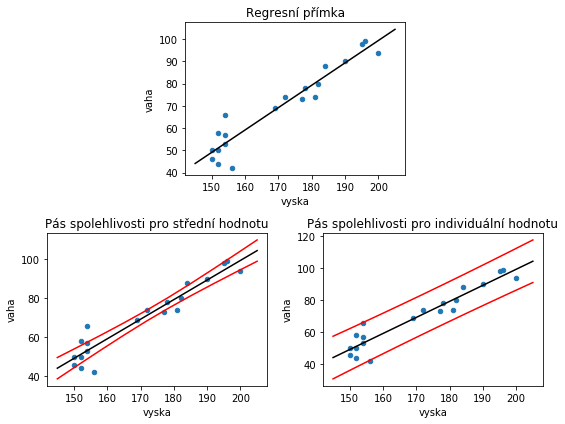
\includegraphics[width=.9\linewidth]{./obipy-resources/uPYyXq.png}
\end{center}
\end{document}